The experiments were conducted as follows. Training consisted of nine example grasps, executed in simulation, with a human in control. These nine grasps were grouped into three grasp types (rim, pinch, and handle). The rim and pinch grasp types were trained on the colander object, and the handle grasp type was demonstrated on the saucepan.

\begin{figure}
 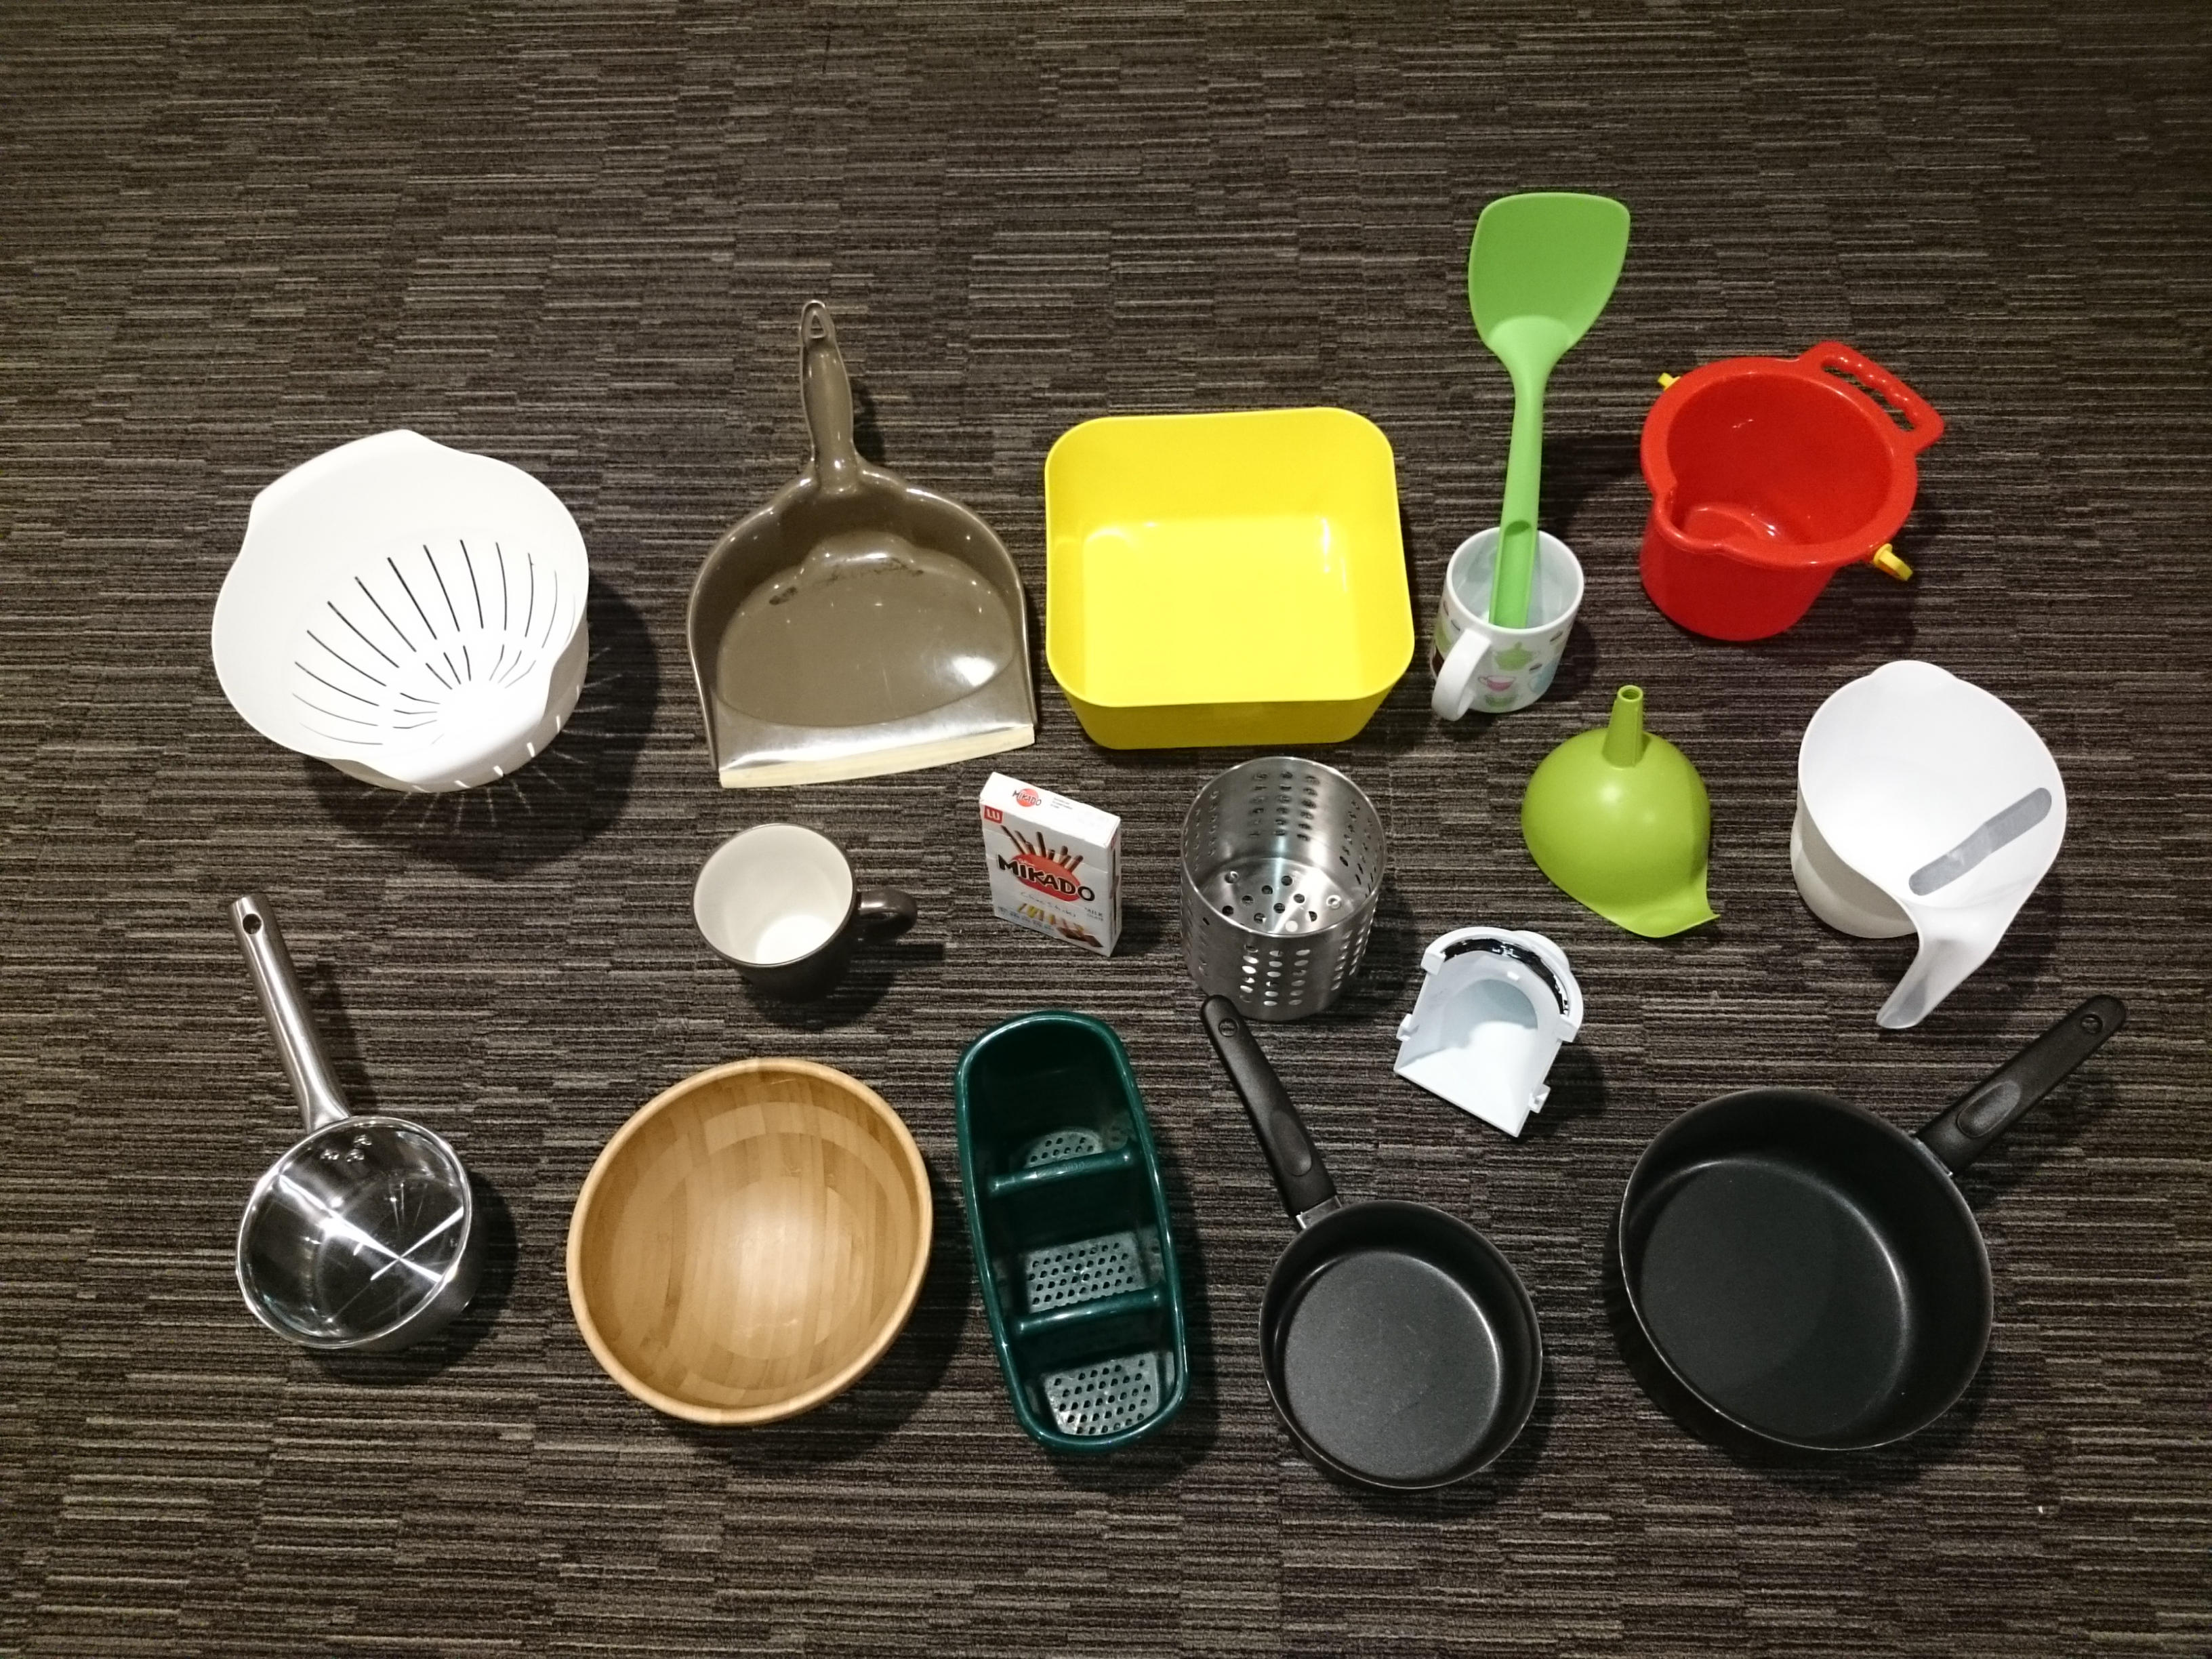
\includegraphics[width=0.9\columnwidth]{images/object_set}
 \caption{The two training objects are on the far left. The testing objects on the right. 12 from 15 test grasps on novel objects were successful.}
 \label{fig:test}
\end{figure}

\begin{figure*}
\newcommand{\w}{0.18\linewidth}
 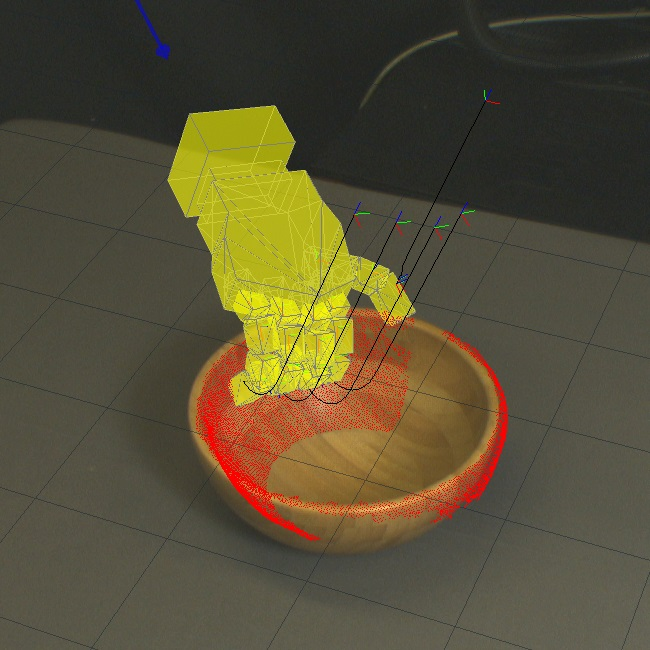
\includegraphics[width=0.45\tw]{images/query/bowllarge-1-s}
  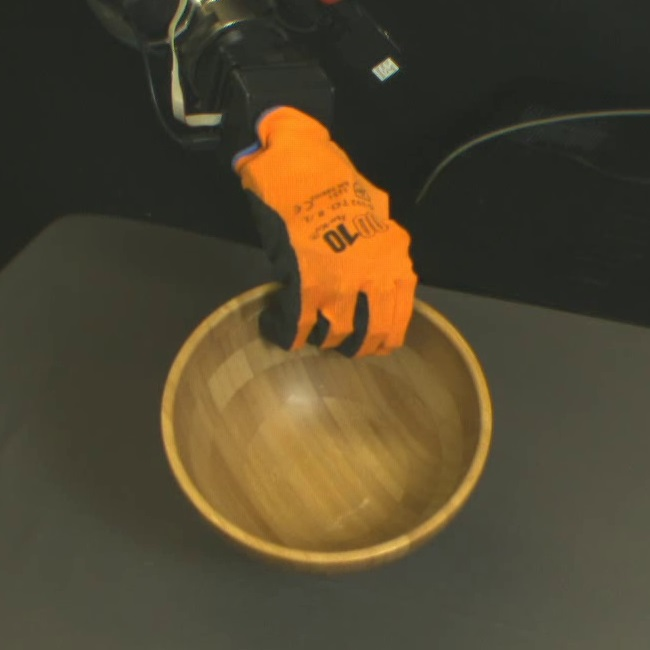
\includegraphics[width=0.45\tw]{images/exec/bowllarge-s}
 \caption{The fifteen test grasps.}
 \label{fig:test}
\end{figure*}
